\section{Metoda odwracania sygnału w czasie}
\label{sec:metoda_tr}

Metoda omawiana w tej sekcji polega na wygenerowaniu sygnału który po przepropagowaniu pewnej odległości sam się skompensuje. Technika kompensacji dyspersji poprzez wygenerowanie sygnału odwróconego w czasie została zaprezentowana w artykule [] [\textcolor{red}{referencja do pialucha}]

\subsection{Podstawy teoretyczne}
Podstawową ideą prezentowanej w tej części pracy techniki kompensacji dyspersji jest wytworzenie sygnału, który poprzez nałożenie składowych częstotliwości w czasie propagacji skompensuje się, tworząc oczekiwany sygnał w pozycji pomiarowej. W przypadku w którym do obiektu wprowadzony zostanie zwykły sygnał sinusoidalny o liniowo zmieniającej się częstotliwości (linear-chirp) zostanie wzbudzone przynajmniej kilka trybów fali prowadzonej. Każdy tryb w każdej z częstotliwości może poruszać się z różną prędkością fazową i grupową. Ze względu na dyspersję sygnał wraz z propagacją będzie stawał się coraz dłuższy a jego amplituda będzie spadać, ponieważ ulegnie on rozproszeniu.  Składowe częstotliwości sygnału odpowiadające najwyższym prędkością grupowym będą znajdować się z przodu, natomiast wolniejsze komponenty będą znajdowały się z tyłu. Podstawa przedstawianej metody polega na założeniu, że tak otrzymany sygnał jesteśmy w stanie odwrócić w czasie, tak aby komponenty o mniejszej prędkości znalazły się z przodu sygnału a komponenty o większej prędkości znalazły się z tyłu. Wzbudzenie obiektu tak przygotowanym sygnałem da w odpowiedzi sygnał skompensowany tej samej postaci co pierwotne wzbudzenie. Skuteczność metody można wykazać analitycznie. Przyjijmy, że sygnał zastosowany do wzbudzenia pręta zostanie zastosowany w punkcie $x = 0$ i będzie to sygnał $f(t)$. Sygnał wzbudzający w dziedzinie częstotliwości możemy zapisać jako:
\begin{equation}
[F(\omega)_{x=0}=\int\limits_{-\int}^{\int}]f(t)e^{-i\omega t}dt \label{eq:F(omega)_x=0}
\end{equation}
Jeśli przez nasz obiekt propaguje jedna postać fali to w punkcie $x=L$ można tę funkcję zapisać jako:

\begin{equation}
[F(\omega)_{x=L}=\int\limits_{-\int}^{\int}]f(t)e^{-i(\omega t - kL}dt \label{eq:F(omega)_x=L}
\end{equation}

gdzie liczba falowa k jest funkcją częstotliwości $\omega$  , która jest opisana za pomocą krzywej dyspersji dla danego trybu fali. Równania (\ref{eq:F(omega)_x=0}) oraz (\ref{eq:F(omega)_x=L}) można powiązać funkcją przejścia $H(\omega)$ co można zapisać jako:
\begin{equation}
H(\omega) = \frac{[F(\omega)]_{x=L}}{[F(\omega)]_{x=0}} \label{eq:h(omega)}
\end{equation}

Zakładając, że chcemy uzyskać sygnał $g(t)$, którego transformata Fouriera to $G(\omega)$ przy ($x = L$) wtedy wymagany sygnał wejściowy ($x = 0$) $Y(\omega)$:
\begin{equation}
Y(\omega) = \frac{G(\omega)}{H(\omega)} = G(\omega)[H(\omega)]^{-1} \label{eq:Y(omega)}
\end{equation}
Sygnał w dziedzinie czasu y(t) jaki musi zostać wprowadzony do badanego pręta w punkcie $x=0$ aby uzyskać odebrany sygnał $g(t)$ w punkcie $x=L$ można uzyskać z odwrotnej transformaty Fouriera, co pokazuje równanie (\ref{eq:Y(omega)}):
\begin{equation}
y(t) = \frac{1}{2\pi}\int\limits_{-\infty}^{\infty}\frac{G(\omega)}{H(\omega)}e^{i\omega t}d\omega \label{eq:y(t)}
\end{equation}

W prostym przypadku gdy analizujemy pojedynczą postać fali prowadzonej:
\begin{equation}
[H(\omega)]^{-1} = e^{-ikL} = e^{-i\omega L/c}
\end{equation}
\begin{equation}
y(t) = \frac{1}{2\pi}\int\limits_{-\infty}^{\infty}G(\omega)e^{-i\omega (L/c - t)}d\omega
\end{equation}

Przyjmując, że sygnał w domenie czas $g(t)$ jest aplikowany w punkcie $x = 0$ sygnał $y^*(t)$ w punkcie x = L można zapisać jako:
\begin{equation}
y^*(t) = \frac{1}{2\pi}\int\limits_{-\infty}^{\infty}G(\omega)e^{-i\omega (L/c + t)}d\omega
\end{equation}

Technika kompensacji w tym przypadku polega na odebraniu sygnału $y*(t)$ w przedziale czasowym $t\in [0,T]$ w którym cała paczka falowa zostanie odebrana przez odbiornik. Następnie sygnał zostaje odwrócony w czasie. Otrzymany w ten sposób sygnał może być zaaplikowany do badanego pręta. W trakcie propagacji zostanie on skompensowany do fali o kształcie takim jak kształt sygnału $g(t)$

\subsection{Implementacja numeryczna}
W ramach niniejszej pracy, omawiana metoda została zaimplementowana do aplikacji. Podstawa jej działania opiera się na znajomości krzywych dyspersji. Pierwszym etapem jest wygenerowanie sygnału, jaki chce się uzyskać w wyniku kompensacji. Następnie dzięki zaimplementowanym metodom należy uzyskać przewidywany kształt sygnału po przepropagowaniu zadanej odległości oraz odrócenie go w czasie. Sygnał otrzymany z tak przygotowanego sygnału wejściowego powinien skompensować się na zadanej odległości. Rysunek \ref{fig:kolejne_etapy_TR} przedstawia opisane kroki na przykładzie chirpa.
\begin{figure}[h]
\centering
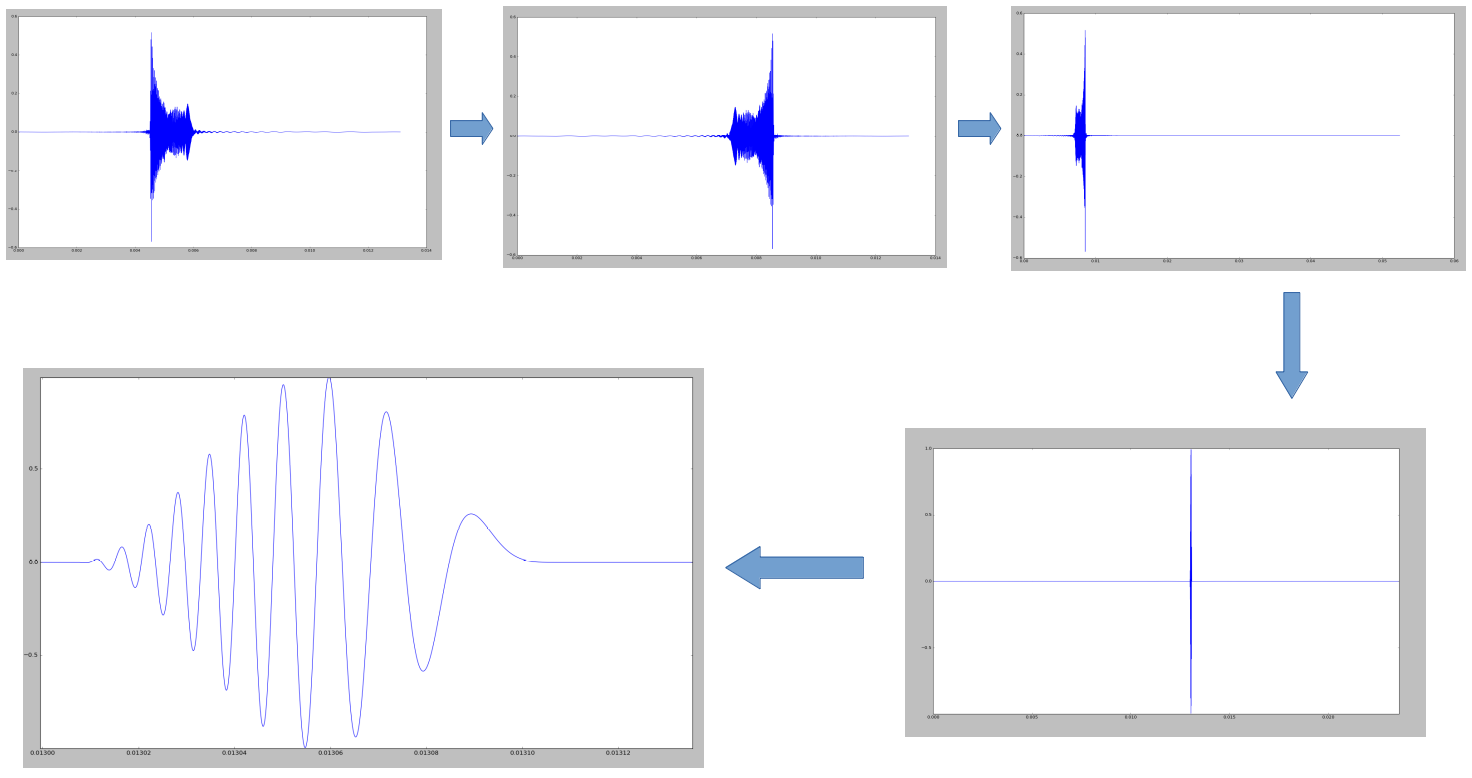
\includegraphics[width=14cm]{Zdjecia/4/algorytm_komp_tr}
\caption{Algorytm kompensacji odwracania czasu}
\label{fig:kolejne_etapy_TR}
\end{figure}

W zaprezentowanym przykładzie odwrócony w czasie sygnał został dodatkowo wypełniony zerami. Zabieg ten został zastosowany, ponieważ całość została przeprowadzona w ramach symulacji i wypełnienie sygnału było zabiegiem niezbędnym do przeprowadzenia prawidłowej symulacji propagacji. Przedstawiana metoda pozwala zatem wygenerować sygnał kompensujący się na zadanej odległości do fali o oczekiwanym kształcie. Pozwala na propagowanie zarówno pojedynczego trybu jaki nałożonych wielu postaci. Jednak aby móc stosować tę motodę konieczna jest znajomość długości ścieżki propagacji sygnału. Jeżeli ściażka propagacji ulegnie zmianie, konieczne jest wygenerowanie nowego sygnału adekwatnego do aktualnego badanego obiektu. W przypadku w którym podczas propagacji następowałyby dodatkowe odbicia, na przykład w sytuacji, w której fala propagujące przez dwa pręty złączone ze sobą, część energii odbiła by się od łączenia a część przepropagowała przez drugi pręt i odbiła się na końcu. Stworzenie sygnału kompensującego się w takiej sytuacji byłoby bardziej skomplikowane i nie zostało opisane w tej pracy. Rysunek \ref{fig:rozne_odl} prezentuje przykład fali przygotowanej do kompensacji po 4 metrach propagacji. 

\begin{figure}[h]
\centering
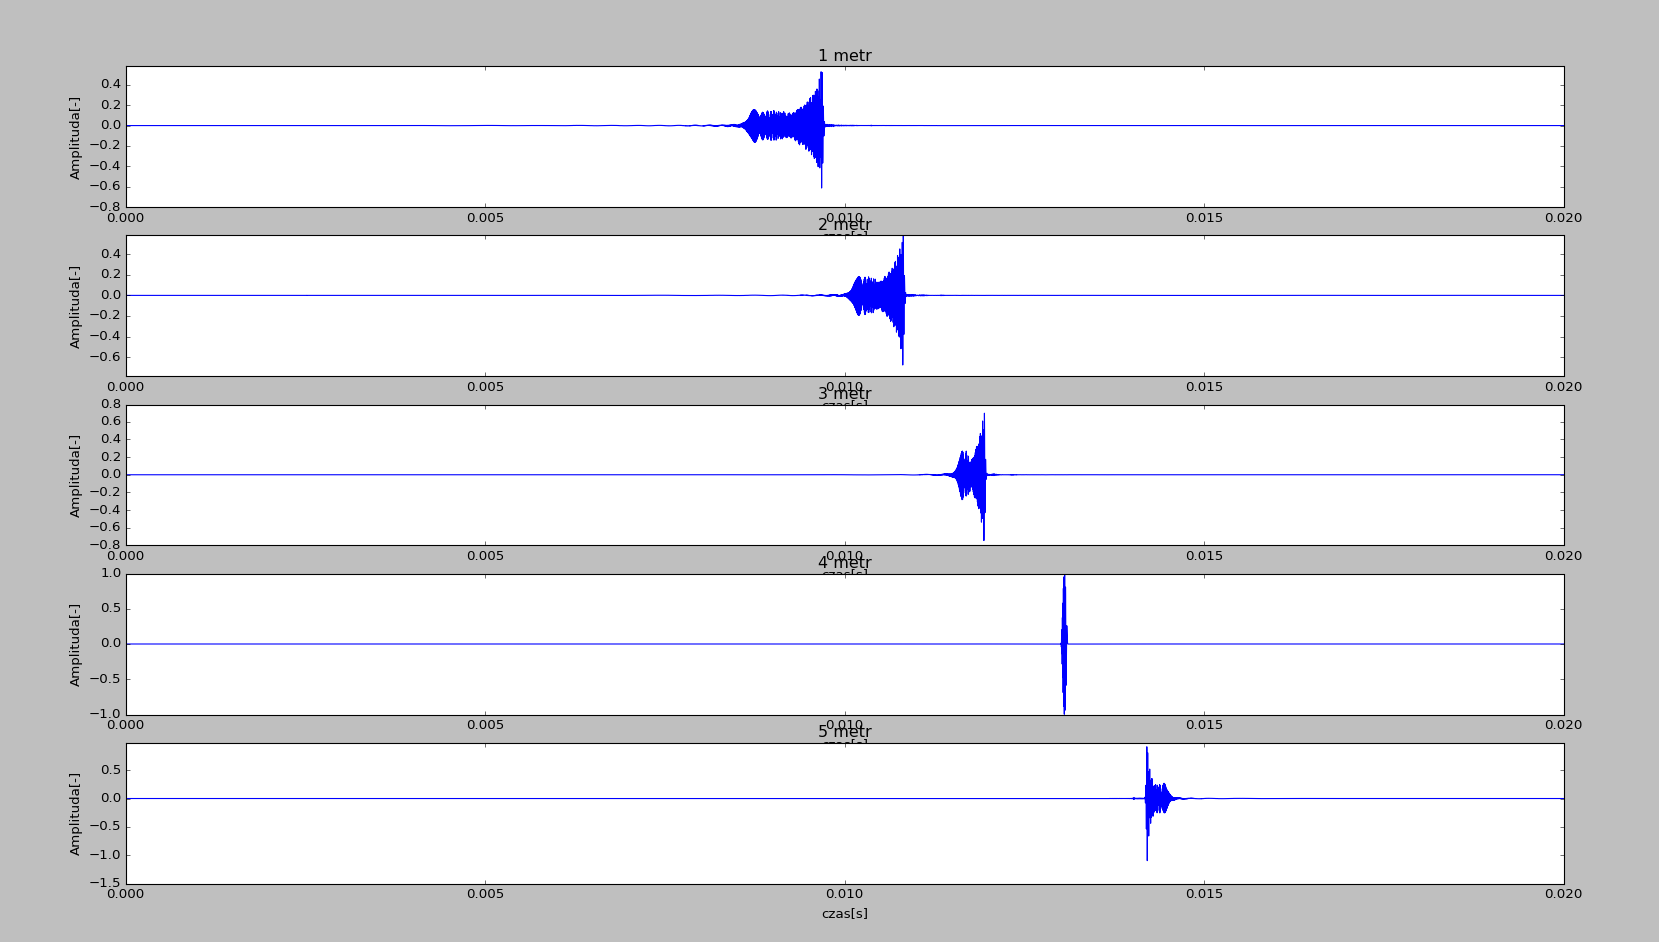
\includegraphics[width=14cm]{Zdjecia/4/porownanie_roznych_odleglosci_time_reversal}
\caption{Sygnał przygotowany do kompensacji po 4 metrach propagacji przedstawiony kolejno po 1, 2, 4 i 5 metrach propagacji}
\label{fig:rozne_odl}
\end{figure}

Jak łatwo zauważyć wprowadzony sygnał kompensuje się tylko i wyłącznie po przepropagowaniu założonej odległości. wraz z oddalaniem się od punktu, w którm przewidziany był odbiornik efekt dyspersji się nasila. Tak więc zarówno przed jak i za założonym punktem odbioru odebrany sygnał byłby rozproszony. Metoda ta może służyć do przeprowadzania nieniszczących testów obiektów o znanej charakterystyce przejścia. W sytuacji w której w strukturze nie będzie żadnych uszkodzeń otrzymywany sygnał będzie skompensowany. Natomiast gdy pojawią się uszkodzenia, nieciągłości w strukturze spowodują odbicie fali i skrócenie ścieżki propagacji co da informację o uszkodzeniach. 

\subsection{Wybrane wyniki z symulacji}
Rysunek \ref{fig:sygnal we} przedstawiono sygnał przekazany do funkcji, jako ten, do którego sygnał ma się skompensować po przepropagowaniu zadanej odległości
\begin{figure}[h]
\centering
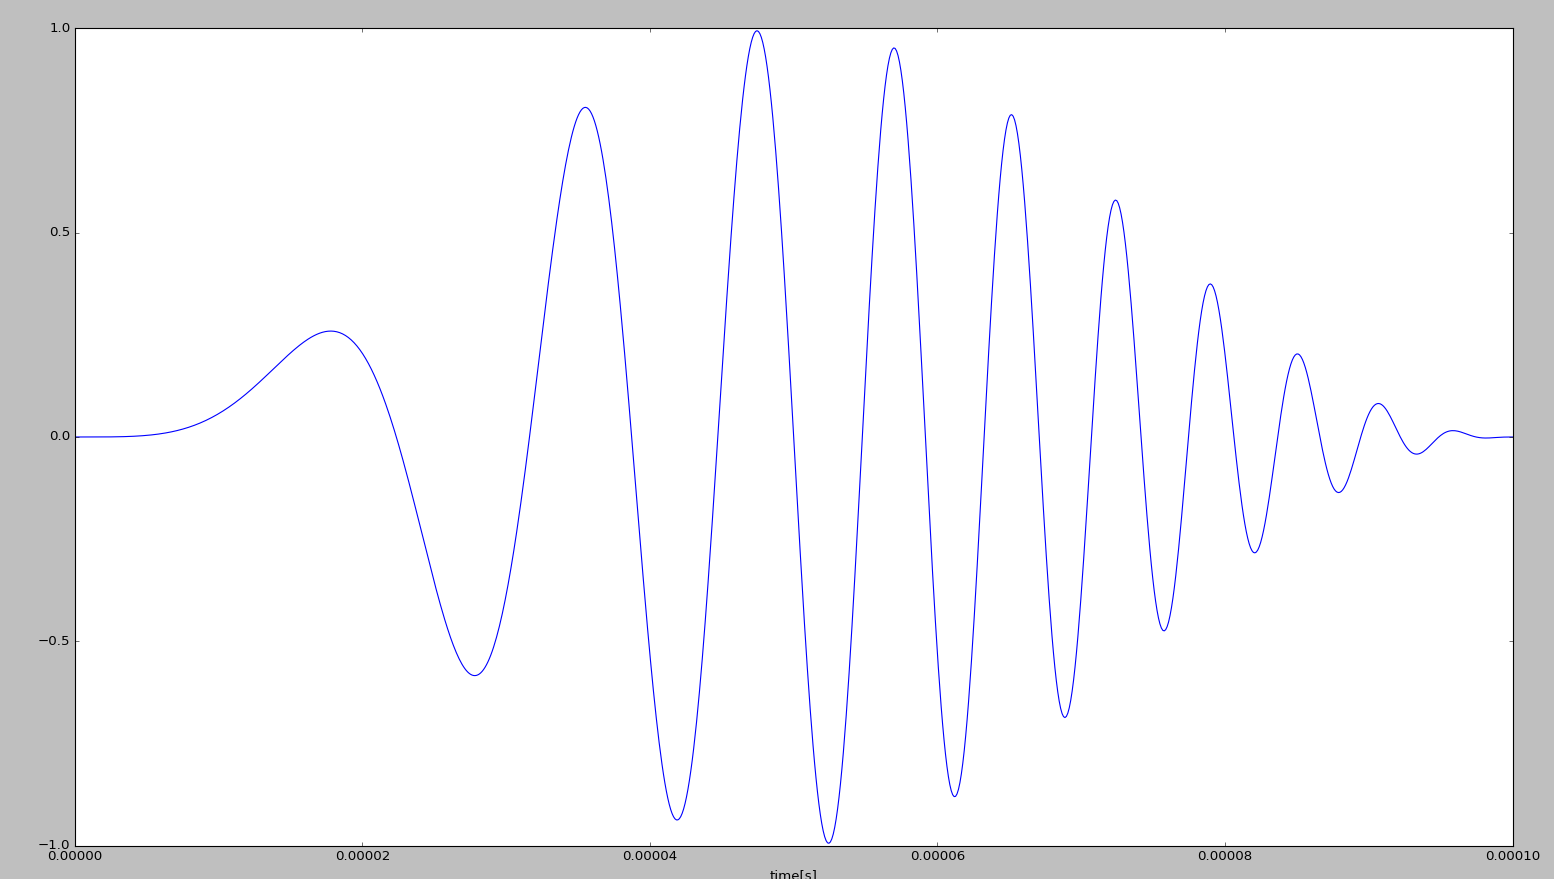
\includegraphics[width=14cm]{Zdjecia/4/test_chirp}
\caption{Algorytm kompensacji odwracania czasu}
\label{fig:sygnal we}
\end{figure}
Wygenerowany przez aplikację sygnał jest różny dla różnych zadanych odległości. Obrazuje to rysunek \ref{fig:rozne_odl} na którym przedstawiono sygnały mające się skompensować odpowiednio po 1 2 3 4 metrach, gdy propagują pierwsze cztery postaci fali prowadzonej. 
\begin{figure}[h]
\centering
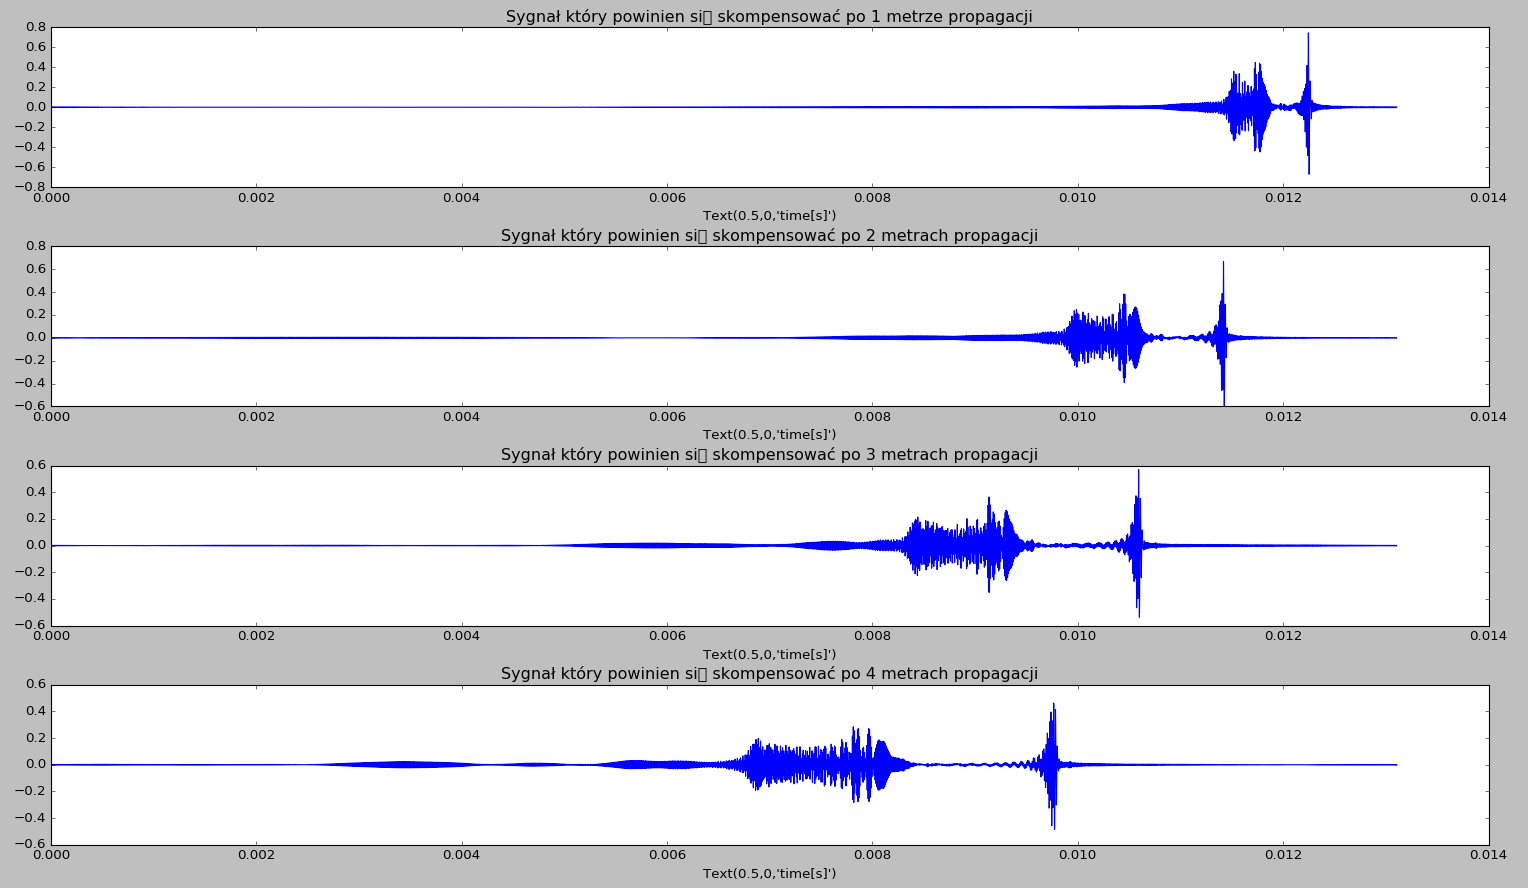
\includegraphics[width=14cm]{Zdjecia/4/tr_przykl}
\caption{Sygnał przygotowany do kompensacji po odpowiedno 1,2,3 oraz 4 metrach}
\label{fig:rozne_odl}
\end{figure}
Sygnał jest też różny dla różnej ilości propagujących trybów, rysunek \ref{fig:rozne_tryby}
\begin{figure}[h]
\centering
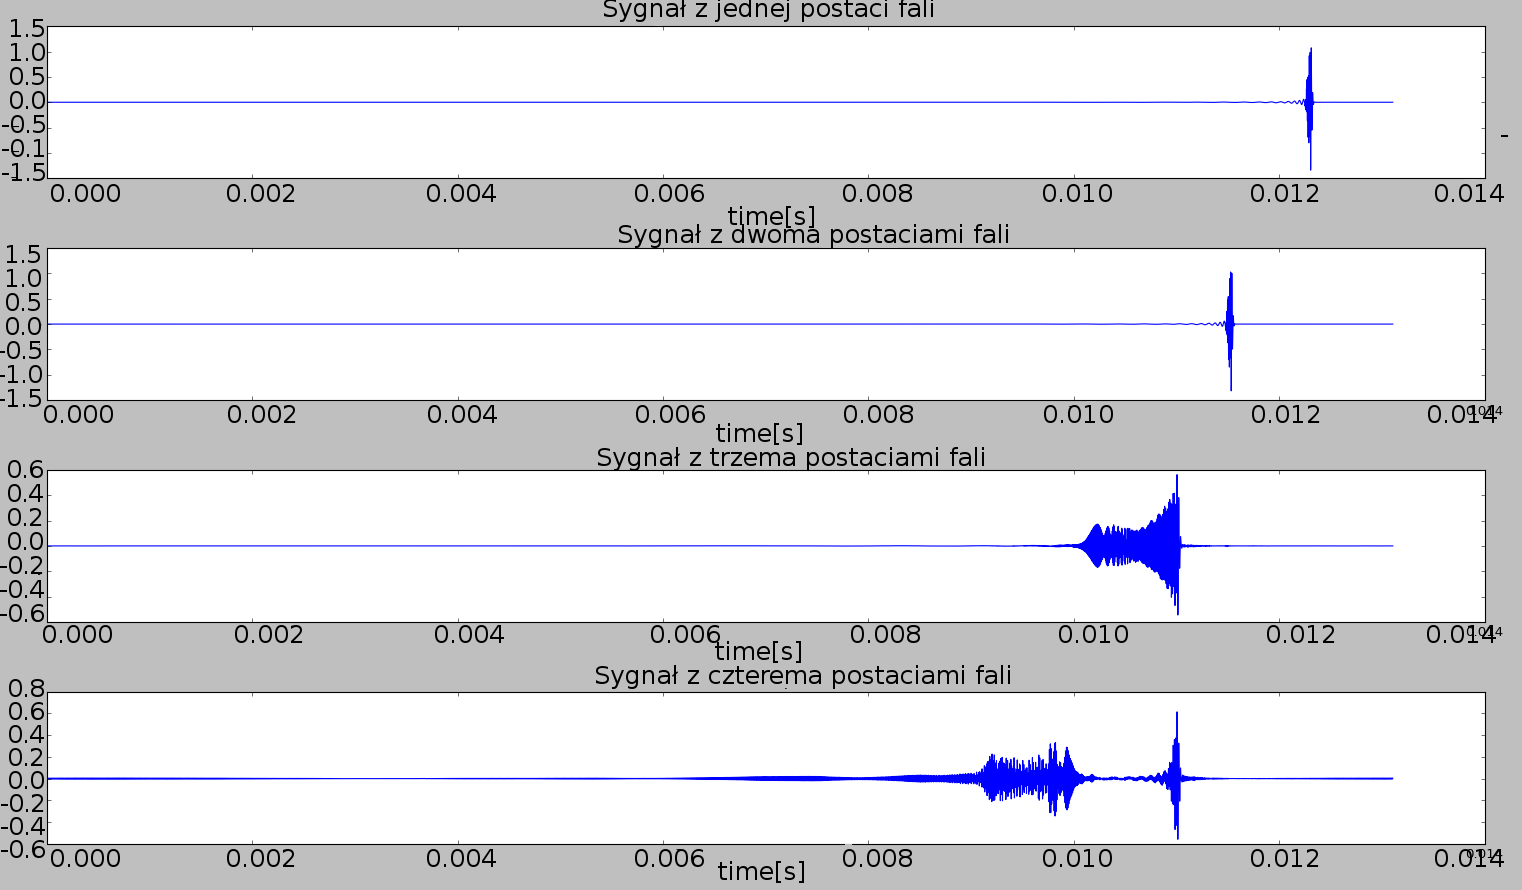
\includegraphics[width=14cm]{Zdjecia/4/TR-rozna_ilosc_modow}
\caption{Sygnał przygotowany do kompensacji po 2,5 metra propagacji zawierający kolejno 1,2,3 oraz 4 postaci fali prowadzonej}
\label{fig:rozne_tryby}
\end{figure}
Tak wygenerowane sygnały zostały przetestowane przez propagację w symulacji. Rysunek \ref{fig:100} ilustruje jak ważna jest znajomość długości ścieżki propagacji. Jeśli sygnał przebędzie zbyt krótką lub zbyt długą drogę to odebrany sygnał nie będzie skompensowany.
\begin{figure}[h]
\centering
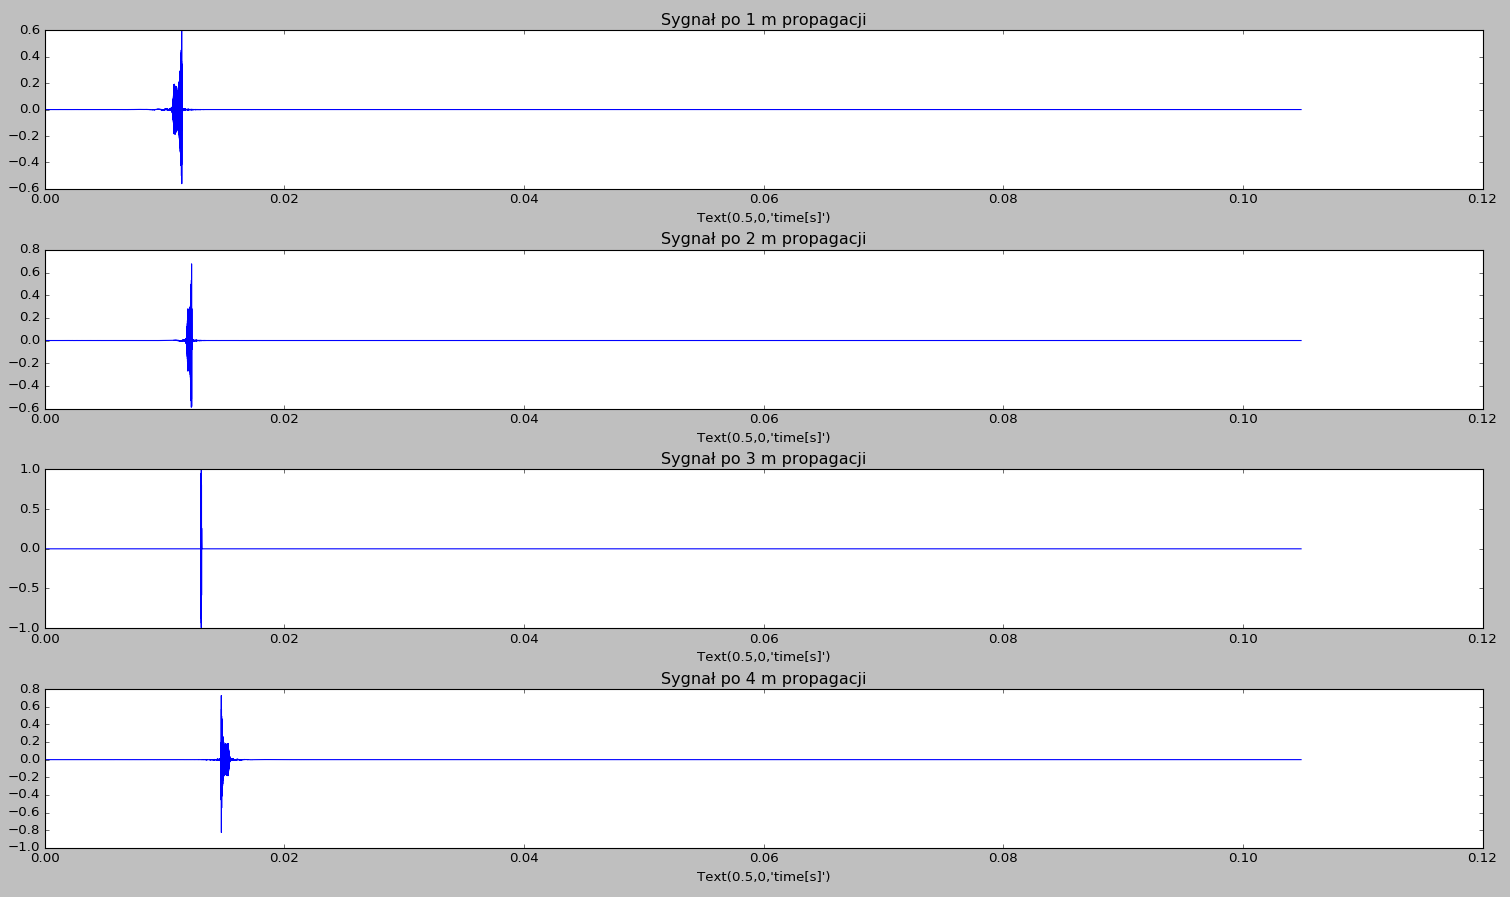
\includegraphics[width=14cm]{Zdjecia/4/obrazek100}
\caption{Sygnał przygotowany do kompensacji po 3 metrach propagacji przepropagowany kolejno o 1,2,3 i 5 metrów}
\label{fig:100}
\end{figure}
Rysunek \ref{fig:skompensowane_TR} ilustruje wyniki symulacji propagacji na odpowiednie odległości sygnałów przedstawinych na rysunku 4.9
\begin{figure}[h]
\centering
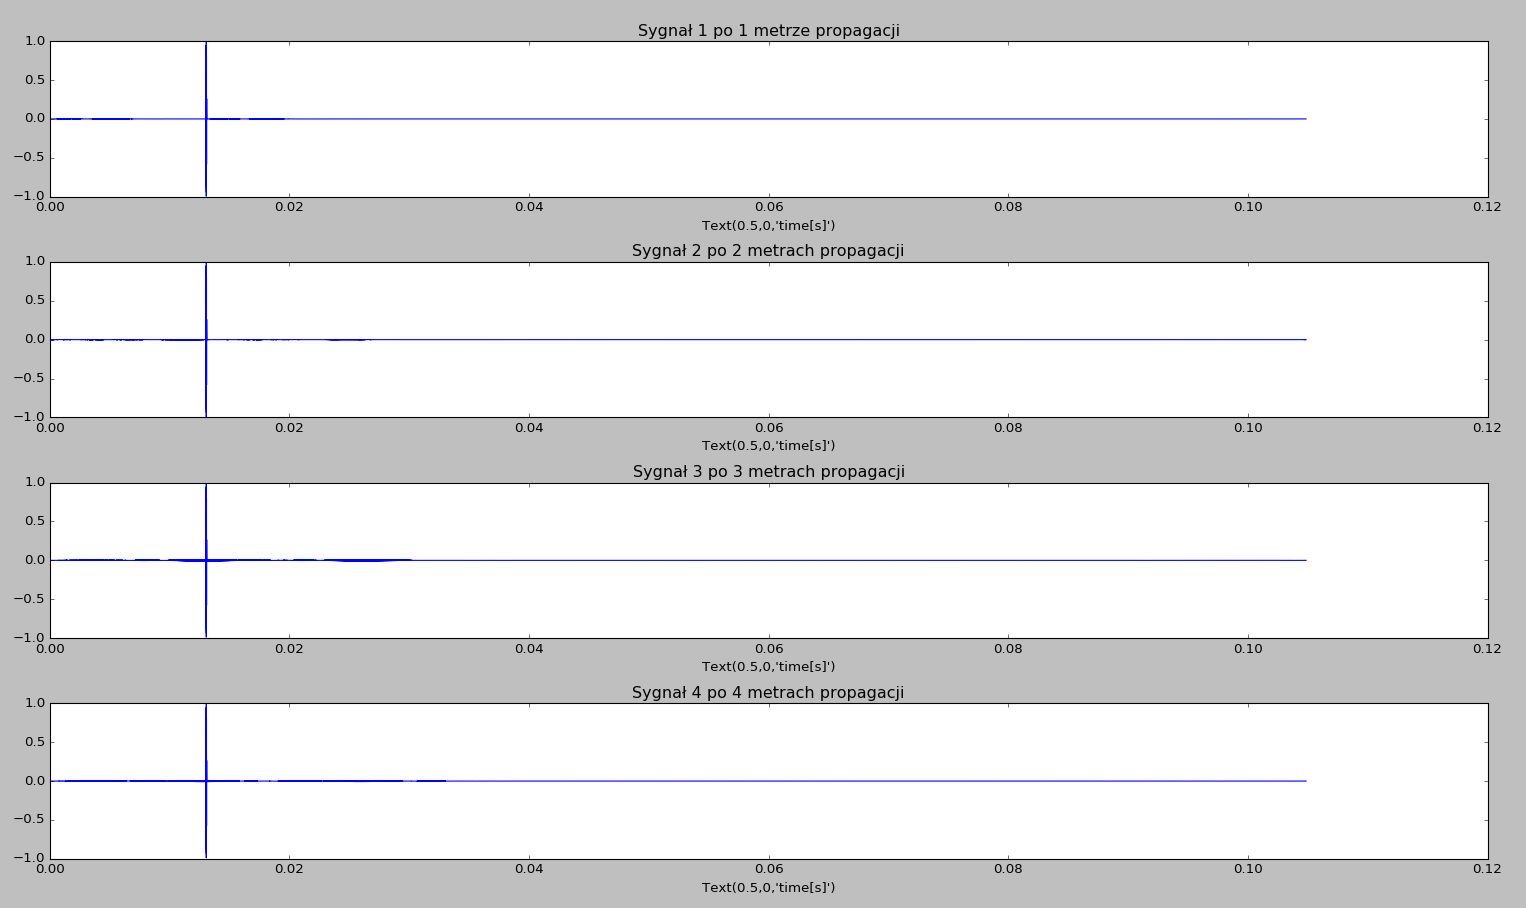
\includegraphics[width=14cm]{Zdjecia/4/skompensowane_TR}
\caption{Sygnały  z rysunu 4.9 po przepropagowaniu odpowiednich odległości}
\label{fig:skompensowane_TR}
\end{figure}

Rysunek \ref{fig:tr_rozna_il_postaci_skomp} ilustruje wyniki  symulacji propagacji sygnałów przedstawionych na rysunku 4.10
\begin{figure}[h]
\centering
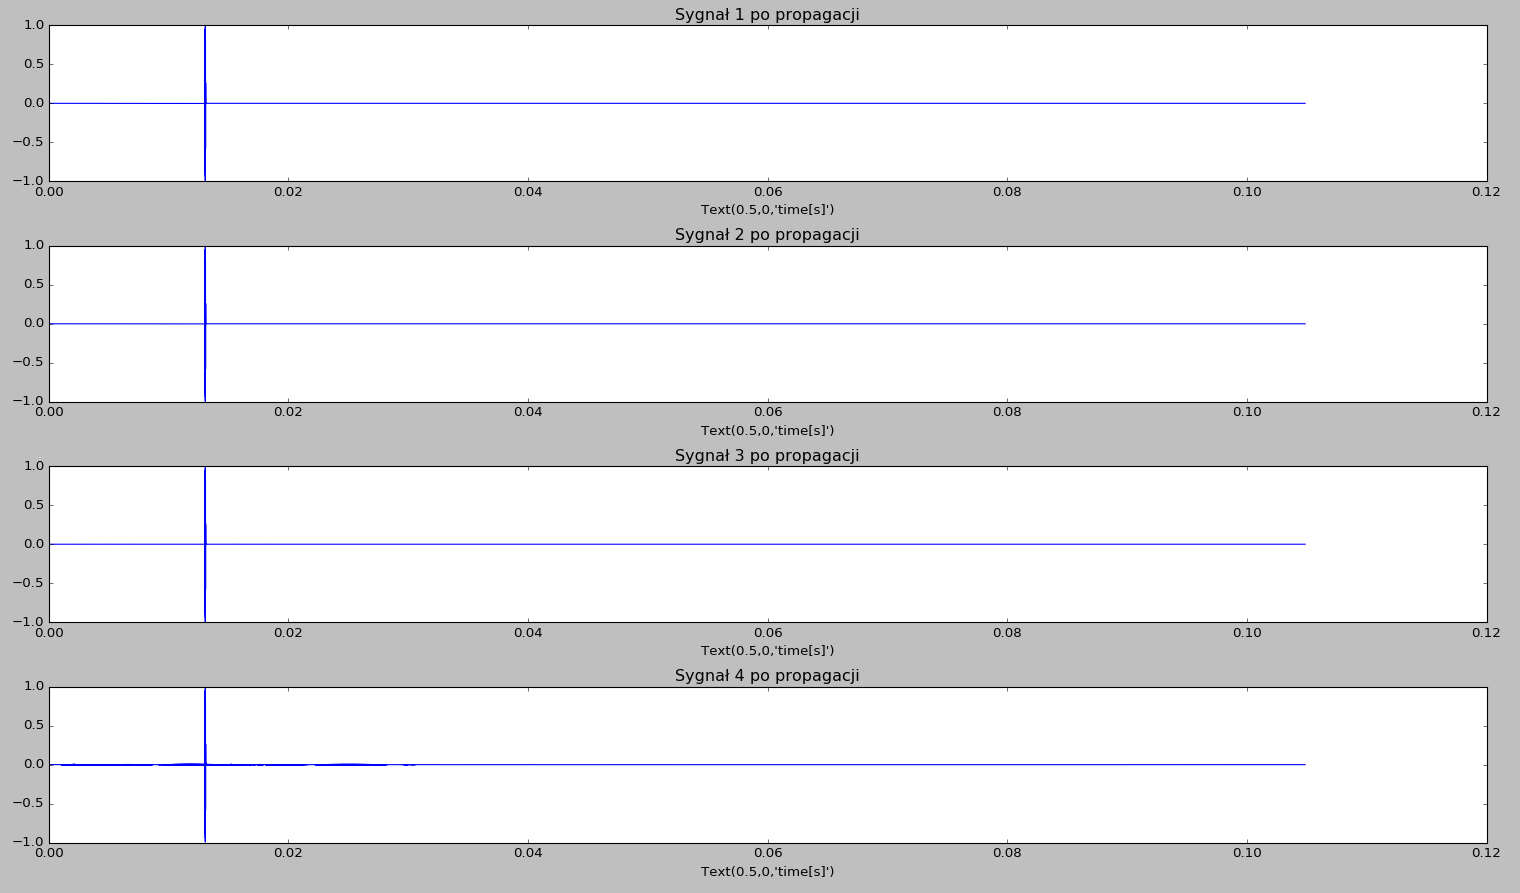
\includegraphics[width=14cm]{Zdjecia/4/tr_rozna_il_postaci_skomp}
\caption{Sygnały  z rysunu 4.10 po przepropagowaniu odpowiedniej odległości}
\label{fig:tr_rozna_il_postaci_skomp}
\end{figure} 